\documentclass[conf]{new-aiaa}
%\documentclass[journal]{new-aiaa} for journal papers
\usepackage[utf8]{inputenc}


%% Packages
\usepackage{graphicx}
\usepackage{amsmath}
\usepackage[version=4]{mhchem}
\usepackage{siunitx}
\usepackage{placeins}
\usepackage{longtable,tabularx}
\usepackage{physics}
\setlength\LTleft{0pt} 


%% User Commands
\newcommand{\FigDir}{./attachments/Figures/}
\newcommand{\TexDir}{./attachments/tex/}

% Math Commands
\newcommand{\mdotf}{\dot{m}_f}
\newcommand{\Nb}{\mathcal{N}}

\title{Theory Guide}

\author{Isaiah M. Helt\footnote{Aerodynamicist, Launch Vehicles Division, ihelt3@gatech.edu}}
\affil{Northrop Grumman, 1575 S Price Rd, Chandler, AZ 85286}

\begin{document}

\maketitle


%%%%%%%%%%%%%%%%%%%%%%%%%%%%%%%%%%%%%%%%%%%%%%%%%%%%%%%%%%%%%%%%%%%

%%%%%%% 				       Abstract 					%%%%%%%

%%%%%%%%%%%%%%%%%%%%%%%%%%%%%%%%%%%%%%%%%%%%%%%%%%%%%%%%%%%%%%%%%%%
\begin{abstract}
These instructions give you guidelines for preparing papers for AIAA Technical Papers using \LaTeX{}. Define all symbols used in the abstract. Do not cite references in the abstract. The footnote on the first page should list the Job Title and AIAA Member Grade for each author, if known Authors do not have to be AIAA members.
\end{abstract}


%%%%%%%%%%%%%%%%%%%%%%%%%%%%%%%%%%%%%%%%%%%%%%%%%%%%%%%%%%%%%%%%%%%

%%%%%%% 				   Nomenclature 					%%%%%%%

%%%%%%%%%%%%%%%%%%%%%%%%%%%%%%%%%%%%%%%%%%%%%%%%%%%%%%%%%%%%%%%%%%%
\section{Nomenclature}

{\renewcommand\arraystretch{1.0}
\noindent\begin{longtable*}{@{}l @{\quad=\quad} l@{}}
$u_i$  		& $i^\text{th}$-velocity component \\
$\mu$ 		& dynamic viscosity \\
$\nu$ 		& kinematic viscosity \\
$\nu_T$ 	& kinematic Eddy viscosity
\end{longtable*}}


%%%%%%%%%%%%%%%%%%%%%%%%%%%%%%%%%%%%%%%%%%%%%%%%%%%%%%%%%%%%%%%%%%%

%%%%%%% 				   Introduction 					%%%%%%%

%%%%%%%%%%%%%%%%%%%%%%%%%%%%%%%%%%%%%%%%%%%%%%%%%%%%%%%%%%%%%%%%%%%
\clearpage
\FloatBarrier
\section{Introduction}


%%%%%%%%%%%%%%%%%%%%%%%%%%%%%%%%%%%%%%%%%%%%%%%%%%%%%%%%%%%%%%%%%%%

%%%%%%% 				       Mesh       					%%%%%%%

%%%%%%%%%%%%%%%%%%%%%%%%%%%%%%%%%%%%%%%%%%%%%%%%%%%%%%%%%%%%%%%%%%%
\clearpage
\FloatBarrier
\section{Mesh}



%%%%%%%%%%%%%%%%%%%%%%%%%%%%%%%%%%%%%%%%%%%%%%%%%%%%%%%%%%%%%%%%%%%

%%%%%%% 			   Boundary Conditions 					%%%%%%%

%%%%%%%%%%%%%%%%%%%%%%%%%%%%%%%%%%%%%%%%%%%%%%%%%%%%%%%%%%%%%%%%%%%
\clearpage
\FloatBarrier
\section{Boundary Conditions}

\subsection{Viscous Wall}



\subsection{Freestream}



\subsection{Inlet}



\subsection{Outlet}


%%%%%%%%%%%%%%%%%%%%%%%%%%%%%%%%%%%%%%%%%%%%%%%%%%%%%%%%%%%%%%%%%%%

%%%%%%% 					Turbulence 						%%%%%%%

%%%%%%%%%%%%%%%%%%%%%%%%%%%%%%%%%%%%%%%%%%%%%%%%%%%%%%%%%%%%%%%%%%%
\clearpage
\FloatBarrier
\section{Turbulence}

This section will detail turbulence theory and modeling in the LUNA code framework. 

\subsection{Reynolds-Averaged Navier Stokes (RANS) Models}

Reynolds-Averaged Navier Stokes models are based on either solving for the mean flow using the eddy viscosity hypothesis, or close the Reynolds stress tensors, $u_iu_j$. At the moment, LUNA only implements eddy viscosity models. 

The turbulent viscosity hypothesis, or eddy viscosity hypothesis, assumes that the turbulent effects can be modeled via a dissipative eddy viscosity term, denoted $\nu_T = \mu_T / \rho$ in the Navier Stokes equations. Therefore, the key to solving the closure problem in eddy viscosity models is determining the eddy viscosity. Note that $\nu_T$ is a property of the flow, not the fluid (like the standard viscosity $\nu$).

\begin{equation}
\langle u_i u_j \rangle = \frac{2}{3} k \delta_{ij} - \nu_T \left[ \pdv{\overline{U_i}}{x_j} + \pdv{\overline{U_j}}{x_i} \right]  \label{eddyViscosityHypothesis}
\end{equation}

The eddy viscosity model makes two major assumptions:

\begin{enumerate}
\item The Deviatoric/anisotropic part of the Reynolds stress tensor is treated as a function of local mean strain rates only (i.e. in eq. \ref{eddyViscosityHypothesis}, LHS = RHS for all $i$, $j$ in isotropic turbulence)
\item The relationship between the Reynolds stress and the mean strain rates are linearly related by a single scalar
\end{enumerate}


\subsubsection{Spalart-Allmaras}

Spalart-Allmaras is a low-Reynolds number one equation RANS turbulence model. In other words, one transport equation is required to be solved to determine the eddy viscosity. For a general compressible flow, the eddy viscosity is given as 

\begin{equation}
\mu_T = \rho f_{v1} \tilde{\nu}
\end{equation}

\noindent where 

\begin{itemize}
\item $\rho$ is the density
\item $f_{v1}$ is a damping function 
\item $\tilde{\nu}$ is a modified diffusivity
\end{itemize}

\noindent The damping function is:

\begin{equation}
f_{\nu 1} = \frac{\chi^3}{\chi^3 + c_{\nu1}^3}
\end{equation}

\noindent where:

\begin{equation}
\chi = \frac{\tilde{\nu}}{\nu}
\end{equation}

\noindent The transport equation for the modified diffusivity $\tilde{\nu}$ is:

\begin{equation}
\pdv{\rho \tilde{\nu}}{t} + \pdv{\rho \tilde{\nu} u_j}{x_j} = \frac{1}{\sigma_{\tilde{\nu}}} \pdv{}{x_j} \left[ \left(\mu + \rho \tilde{\nu} \right) \pdv{\tilde{\nu}}{x_j} \right] + P_{\tilde{\nu}} + S_{\tilde{\nu}} \label{SA_transport}
\end{equation}

\noindent where:

\begin{itemize}
\item $u_i$ is the mean velocity
\item $\sigma_{\tilde{\nu}}$ is a model coefficient
\item $\mu$ is the dynamic viscosity
\item $P_{\tilde{\nu}}$ is the production term
\item $S_{\tilde{\nu}}$ is source term
\end{itemize}

\noindent Note that using the continuity equation, eq. \ref{SA_transport} is equivalent to:

\begin{equation}
\rho \left[ \pdv{\tilde{\nu}}{t} + u_j \pdv{\tilde{\nu}}{x_j} \right] = \frac{1}{\sigma_{\tilde{\nu}}} \pdv{}{x_j} \left[ \left(\mu + \rho \tilde{\nu} \right) \pdv{\tilde{\nu}}{x_j} \right] + P_{\tilde{\nu}} + S_{\tilde{\nu}}
\end{equation}




%%%%%%%%%%%%%%%%%%%%%%%%%%%%%%%%%%%%%%%%%%%%%%%%%%%%%%%%%%%%%%%%%%%

%%%%%%% 				Solver Algorithms 					%%%%%%%

%%%%%%%%%%%%%%%%%%%%%%%%%%%%%%%%%%%%%%%%%%%%%%%%%%%%%%%%%%%%%%%%%%%
\clearpage
\FloatBarrier
\section{Solver Algorithms}


%%%%%%%%%%%%%%%%%%%%%%%%%%%%%%%%%%%%%%%%%%%%%%%%%%%%%%%%%%%%%%%%%%%
%% SIMPLE
\subsection{SIMPLE: Semi-Implicit Method for Pressure Linked Equations}


%------------------------------------------------------------------
\FloatBarrier
\subsubsection{Theory}

\begin{figure}
\centering
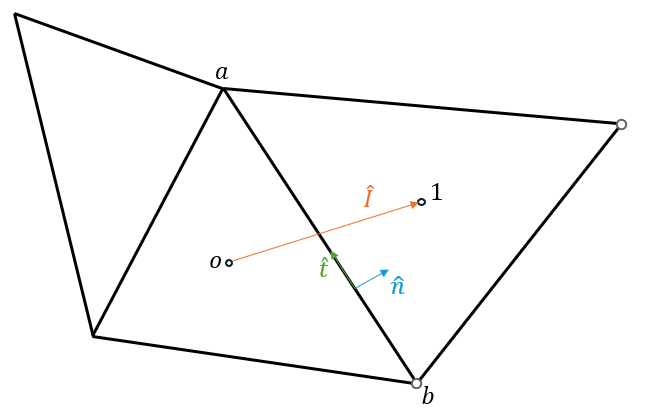
\includegraphics[width=0.7\textwidth]{\FigDir SolverAlgorithms/SIMPLE/MeshRelations.PNG}
\caption{\label{fig:MeshRelations}SIMPLE Algorithm Mesh Relation Terminology}
\end{figure}


%------------------------------------------------------------------
\FloatBarrier
\subsubsection{Application}

% * * * * * * * * * * * * * * * * * * * * * * * * * * * * * * * * * * * * 
\paragraph{Some Common Expressions}

\begin{equation}
\left.\pdv{p}{x_i}\right|_f n_{i,f} =  \frac{p_{\Nb(f)} - p_o}{\delta_f} + \text{tangential component}
\end{equation}

\begin{equation}
\left.\pdv{p}{x_i}\right|_o = \frac{1}{V_o} \sum_{f} p_f A_f n_{i,f}
\end{equation}

\begin{equation}
p_f = w_o p_o + (1-w_o) p_1
\end{equation}



% * * * * * * * * * * * * * * * * * * * * * * * * * * * * * * * * * * * * 
\paragraph{Momentum Equation}

The linear system to be solved for the momentum equation is given in eq. \ref{eq:SIMPLE_momentum}

\begin{equation}
A_o u_o + \sum_{f} A_{\Nb(f)} u_{\Nb(f)} = Q_o \label{eq:SIMPLE_momentum}
\end{equation}

\noindent where the diagonal elements are given by $A_o$

\begin{equation}
A_o = \sum_{f} \left( \frac{|\mdotf| + \mdotf}{2} + \frac{\mu_f A_f}{\delta_f} \right)
\end{equation}

\noindent and the off-diagonal terms are a result of neighboring cells and are defined by the equation below

\begin{equation}
A_{\Nb(f)} = -\frac{|\mdotf| - \mdotf}{2} - \frac{\mu_f A_f}{\delta_f}
\end{equation}

The right hand side of the momentum equation is a combination of source terms due to pressure ($S_o$), skew terms due to the unstructured nature of the solver ($S_{\text{skew},o}$), and contributions from boundary faces ($S_{bc}$). 

\begin{equation}
Q_o = S_o + S_{\text{skew},o} + S_{bc}
\end{equation}

The skew term is given below. Note that if a pure Cartesian grid is provided to the solver, $\hat{t}_f \cdot \vec{I}_f = 0$, so the skew term goes away.

\begin{equation}
S_{\text{skew},o} = - \sum_{f} \left( \left[ \frac{u_{a(f)}^* - u_{b(f)}^*}{\delta_f} \right] \hat{t}_f \cdot \vec{I}_f \right) \mu_f
\end{equation}

In the $S_{\text{skew},o}$ equation above, the $u^*$ terms represent the nodal velocities, which are calculated explicitly using a distance weighted scheme on the cell face velocities:

\begin{equation}
u^* = w_{i,f}u_{i,o}
\end{equation}

Equation \ref{eq:SIMPLE_pressureSource} shows the contribution due to the pressure source.

\begin{equation}
S_o = - \sum_{f} p_f n_{i,f} A_f \label{eq:SIMPLE_pressureSource}
\end{equation}

The contribution from the boundary faces must also be accounted for in the source terms. Effectively, the boundary face source is due a result of a neighbor cell contribution ($A_{N(f)}$) being moved to the right hand side of the linear system:

\begin{equation}
S_{bc} = u_{bc} \left( \frac{|\mdotf| - \mdotf}{2} + \frac{\mu_f A_f}{\delta_f} \right)
\end{equation}





% * * * * * * * * * * * * * * * * * * * * * * * * * * * * * * * * * * * * 
\paragraph{Pressure Correction Equation}


The pressure correction is calculated by correcting any mass imbalance into the cells, as given by the equation below. 

\begin{equation}
\dot{m}_{imb} = \sum_f \rho_f \underbrace{ \left[ w_f \frac{V_o}{A_o\rvert_o} + (1-w_f) \frac{V_1}{A_o \rvert_1} \right] \left( \left.\pdv{p'}{x_i}\right|_f n_{i,f} \right)}_{ u_{i,f}' n_{i,f}'} A_f \label{eq:massConservation}
\end{equation}

\noindent where $u_{i,f}'$ is the velocity correction and we recall that the pressure gradient can be written as a difference in the cell pressure and neighboring cell pressures:

\begin{equation}
\left.\pdv{p}{x_i}\right|_f n_{i,f} =  \frac{p_{\Nb(f)} - p_o}{\delta_f} + \text{tangential component} \label{eq:pgrad}
\end{equation}

The mass imbalance $\dot{m}_{imb}$, is determined by adding all the mass flux sources coming into the cell:

\begin{equation}
\dot{m}_{imb} = \sum_{f} \mdotf \label{eq:mdotimb}
\end{equation}

Therefore, by plugging equations \ref{eq:pgrad} and \ref{eq:mdotimb} into eq \ref{eq:massConservation}, we can write the mass imbalance equation in terms of cell pressures, their neighbors, and the mass imbalance


\begin{equation}
A_o^p p_o + \sum_{f} A_{\Nb(f)}^p p_{\Nb(f)} = -\dot{m}_{imb}
\end{equation}

\noindent where the coefficients are given as

\begin{equation}
A_o^p = \sum_{f(o)} \left[ w_f \frac{V_o}{A_o\rvert_o} + (1-w_f) \frac{V_1}{A_o\rvert_1} \right] \left( \frac{\rho_f A_f}{\delta_f} \right)
\end{equation}

\begin{equation}
A_{\Nb(f)}^p = - \left[ w_f \frac{V_o}{A_o\rvert_o} + (1-w_f) \frac{V_1}{A_o \rvert_1} \right] \frac{\rho_f A_f}{\delta_f}
\end{equation}

Note that when solving the pressure imbalance equation, the mass imbalance should ultimately reduce to 0, as we are solving for an incompressible flow. Additionally, the pressure correction should ultimately reduce to 0 upon convergence, so it is important to use an initial guess of 0 when solving the pressure correction equation to help with convergence. If a non-zero initial guess is used, the final iteration may have trouble converging.

%Note that the pressure at the boundary must be added as a source to the mass imbalance equation:
%
%\begin{equation}
%p_{N(b),\mathrm{source}} = p_b \left[ w_f \frac{V_o}{A_o\rvert_o} + (1-w_f) \frac{V_1}{A_o \rvert_1} \right] \frac{\rho_f A_f}{\delta_f}
%\end{equation} 


After the pressure has been corrected, a relaxation factor, $\alpha^p_{\mathrm{relax}}$, is applied to help the solver stop from diverging. 

\begin{equation}
p' = \alpha^p_{\mathrm{relax}}p'
\end{equation}

The lower the value of $\alpha^p_{\mathrm{relax}}$, the more stable the solution will be. However, the solution will also converge slower with lower $\alpha_{\mathrm{relax}}$. 




% * * * * * * * * * * * * * * * * * * * * * * * * * * * * * * * * * * * * 
\paragraph{Velocity and Mass Corrections}


Corrections for the cell center velocities: 
\begin{align}
u_o' &= -\frac{1}{A_o \rvert_o} \left. \pdv{p'}{x_i} \right|_o V_o  \\
	 &= - \frac{1}{A_o\rvert_o} \sum_{f} p_f' A_f n_{i,f}
\end{align}

Corrections for the cell face velocities:
\begin{equation}
u_f' = - \left[ w_f \frac{V_o}{A_o\rvert_o} + (1-w_f) \frac{V_1}{A_o\rvert_1} \right] \left. \pdv{p'}{x_i} \right|_f
\end{equation}

Correction to the mass face flux
\begin{align}
\mdotf' &= \rho_f A_f  \left( u_i' n_{i,f} \right) \\
%
&= - \rho_f A_f \left[ w_f \frac{V_o}{A_o\rvert_o} + (1-w_f) \frac{V_1}{A_o\rvert_1} \right] \left( \pdv{p'}{x_i} n_{i,f} \right) \\
%
&= - \rho_f A_f \left[ w_f \frac{V_o}{A_o\rvert_o} + (1-w_f) \frac{V_1}{A_o\rvert_1} \right] \left( \frac{p_{\Nb(f)}' - p_o'}{\delta_f} + S_{\text{tangent}} \right) 
\end{align}

Note that the source term due to the tangential component component of the mass flux ($S_{\text{tangent}}$) is generally neglected as the mass imbalance will ultimately go to zero. Therefore the final solution will not be impacted by the tangential terms, though the convergence may be negatively affected. 

After all of the correction terms have been collected, they can be added to the original values (after being relaxed) in order to get the cell value for the next iteration:

\begin{align}
p &= p + p' \\
u &= u + \alpha^u_{\mathrm{relax}} u' \\
\mdotf &= \mdotf + \alpha^u_{\mathrm{relax}} \mdotf'
\end{align}

Note that because the velocity and mass corrections are linearly related, the same relaxation factor is applied to both systems. 





%%%%%%%%%%%%%%%%%%%%%%%%%%%%%%%%%%%%%%%%%%%%%%%%%%%%%%%%%%%%%%%%%%%

%%%%%%% 						Math 						%%%%%%%

%%%%%%%%%%%%%%%%%%%%%%%%%%%%%%%%%%%%%%%%%%%%%%%%%%%%%%%%%%%%%%%%%%%
\clearpage
\FloatBarrier
\section{Math}

%%%%%%%%%%%%%%%%%%%%%%%%%%%%%%%%%%%%%%%%%%%%%%%%%%%%%%%%%%%%%%%%%%%
%% SIMPLE
\subsection{Linear Algebra}




%------------------------------------------------------------------
\FloatBarrier
\subsubsection{Sparse Matrices}

In an implicit CFD solver, a linear system is formed and solved for all transport equations over every cell. This means a matrix must be created for each each of these systems, which has a size of $n \times n$, where $n$ is the number of cells in the mesh. Obviously, this matrix could quickly become very large and take up a huge amount of memory. However, in these matrices, there are a large number of 0 elements. This fact allows us to cleverly store matrix data to save on memory. The LUNA solver uses a Compressed Sparse Row (CSR) matrix format to save on memory, which is detailed here. 

The CSR matrix stores data in 3 different vectors, which are detailed below. NNZ refers to the number of nonzero elements in a general $m \times n$ matrix, where $m$ is the number of rows, and $n$ is the number of columns.

\begin{itemize}
\item $\vec{v}$: A vector which stores all the non-zero vectors in the matrix (size: NNZ)
\item $\vec{c}$: A vector which stores the column associated each value in the $\vec{v}$ vector (size: NNZ)
\item $\vec{r}$: A vector which always starts with 0, and stores the difference in NNZ elements before and after the row (size: $m+1$)
\end{itemize}

An example is given below for clarity:

\begin{equation}
A = \begin{bmatrix}
0 & 0 & 4 & 0 \\
1 & 0 & 0 & 2 \\
8 & 0 & 0 & 0 \\
0 & 0 & 0 & 0 \\
0 & 7 & 0 & 0
\end{bmatrix}
\end{equation}

\begin{align}
\vec{v} &= \begin{bmatrix} 4 & 1 & 2 & 8 & 7 \end{bmatrix} \\
\vec{c} &= \begin{bmatrix} 3 & 1 & 4 & 1 & 2 \end{bmatrix} \\
\vec{r} &= \begin{bmatrix} 0 & 1 & 3 & 4 & 4 & 5 \end{bmatrix}
\end{align}

The $\vec{v}$ vector is relatively self explanatory in the above example. The $\vec{c}$ vector starts with $3$, indicating the that the value of $4$ is in the $3^\mathrm{rd}$ column, followed by $1$ indicating that the value of $1$ is in the $1^\mathrm{st}$ column, and so on. 

The $\vec{r}$ vector is the least obvious. It starts with 0, as it always does, and then $1$ indicates there was 1 NNZ in the first row. Since there were 2 NNZ in the second row, the third value is $1 + 2 = 3$, where the $1$ is the NNZ in the previous rows. The fourth value is $4$ since there was 1 NNZ in the third row ($1+3=4$), and in the fourth row there are no NNZ, so the vector stays at $4$, finally in the last row there is one last NNZ, so the final value is $4+1=5$. 

While this method does not appear to save much memory for small matrices, it can have a huge impact on the amount of storage used for bigger matrices. 





%%%%%%%%%%%%%%%%%%%%%%%%%%%%%%%%%%%%%%%%%%%%%%%%%%%%%%%%%%%%%%%%%%%

%%%%%%% 				   Conclusions 					    %%%%%%%

%%%%%%%%%%%%%%%%%%%%%%%%%%%%%%%%%%%%%%%%%%%%%%%%%%%%%%%%%%%%%%%%%%%
\section{Conclusion}




%%%%%%%%%%%%%%%%%%%%%%%%%%%%%%%%%%%%%%%%%%%%%%%%%%%%%%%%%%%%%%%%%%%

%%%%%%% 				    Appendix    					%%%%%%%

%%%%%%%%%%%%%%%%%%%%%%%%%%%%%%%%%%%%%%%%%%%%%%%%%%%%%%%%%%%%%%%%%%%
\clearpage
\FloatBarrier
\section*{Appendix}

An Appendix, if needed, should appear before the acknowledgments.



%%%%%%%%%%%%%%%%%%%%%%%%%%%%%%%%%%%%%%%%%%%%%%%%%%%%%%%%%%%%%%%%%%%

%%%%%%% 				  Acknowledgements				    %%%%%%%

%%%%%%%%%%%%%%%%%%%%%%%%%%%%%%%%%%%%%%%%%%%%%%%%%%%%%%%%%%%%%%%%%%%
\section*{Acknowledgments}


%\bibliography{TheoryGuide.bbl}

\end{document}
